\documentclass{article}

% Language setting
% Replace `english' with e.g. `spanish' to change the document language
\usepackage[english]{babel}

% Set page size and margins
% Replace `letterpaper' with `a4paper' for UK/EU standard size
\usepackage[letterpaper,top=2cm,bottom=2cm,left=3cm,right=3cm,marginparwidth=1.75cm]{geometry}

% Useful packages
\usepackage{amsmath}
\usepackage{graphicx}
\usepackage[colorlinks=true, allcolors=blue]{hyperref}
\usepackage[final]{pdfpages}
\usepackage{fancyhdr}
\usepackage{setspace}
\usepackage{enumitem} % Required for customization
\usepackage[shortlabels]{enumitem}
\usepackage{lastpage}

\onehalfspacing
\setlength{\parskip}{0.5\baselineskip}%
\setlength{\parindent}{0pt}%

\renewcommand{\headrulewidth}{.0mm} % header line width

\pagestyle{fancy}
\fancyhf{}
\fancyhfoffset[L]{1cm} % left extra length
\fancyhfoffset[R]{1cm} % right extra length
% \rhead{\today}
% \lhead{\small Permanent Residence Petition for Dr. Yuan Zi}
\rfoot{Page \thepage ~of \pageref*{LastPage}}

% \title{Your Paper}
% \author{You}

\begin{document}

\vspace*{\fill}
\begin{center}

{\bf 
Immigrant Petition for Alien Worker\\
for the Alien with Exceptional Ability in Science (EB2-NIW)
}

\end{center}
\vspace*{\fill}

\begin{center}
TABLE OF CONTENTS
\end{center}
\begin{itemize}
    \item [p. \pageref*{G-1145}] Form G-1145 e-Notification of Application/Petition Acceptance. 
    \item [p. \pageref*{ETA-9089}] Form ETA-9089 Application for Permanent Employment Certification. 
        
    \item [p. \pageref*{I-140}] Form I-140, Immigrant Petition for Alien Worker with the filing fee.
    \item [p. \pageref*{petition}] Immigrant Petition Letter.
    \item [p. \pageref*{exhib}] Exhibits.
\end{itemize}

\clearpage
\label{G-1145}
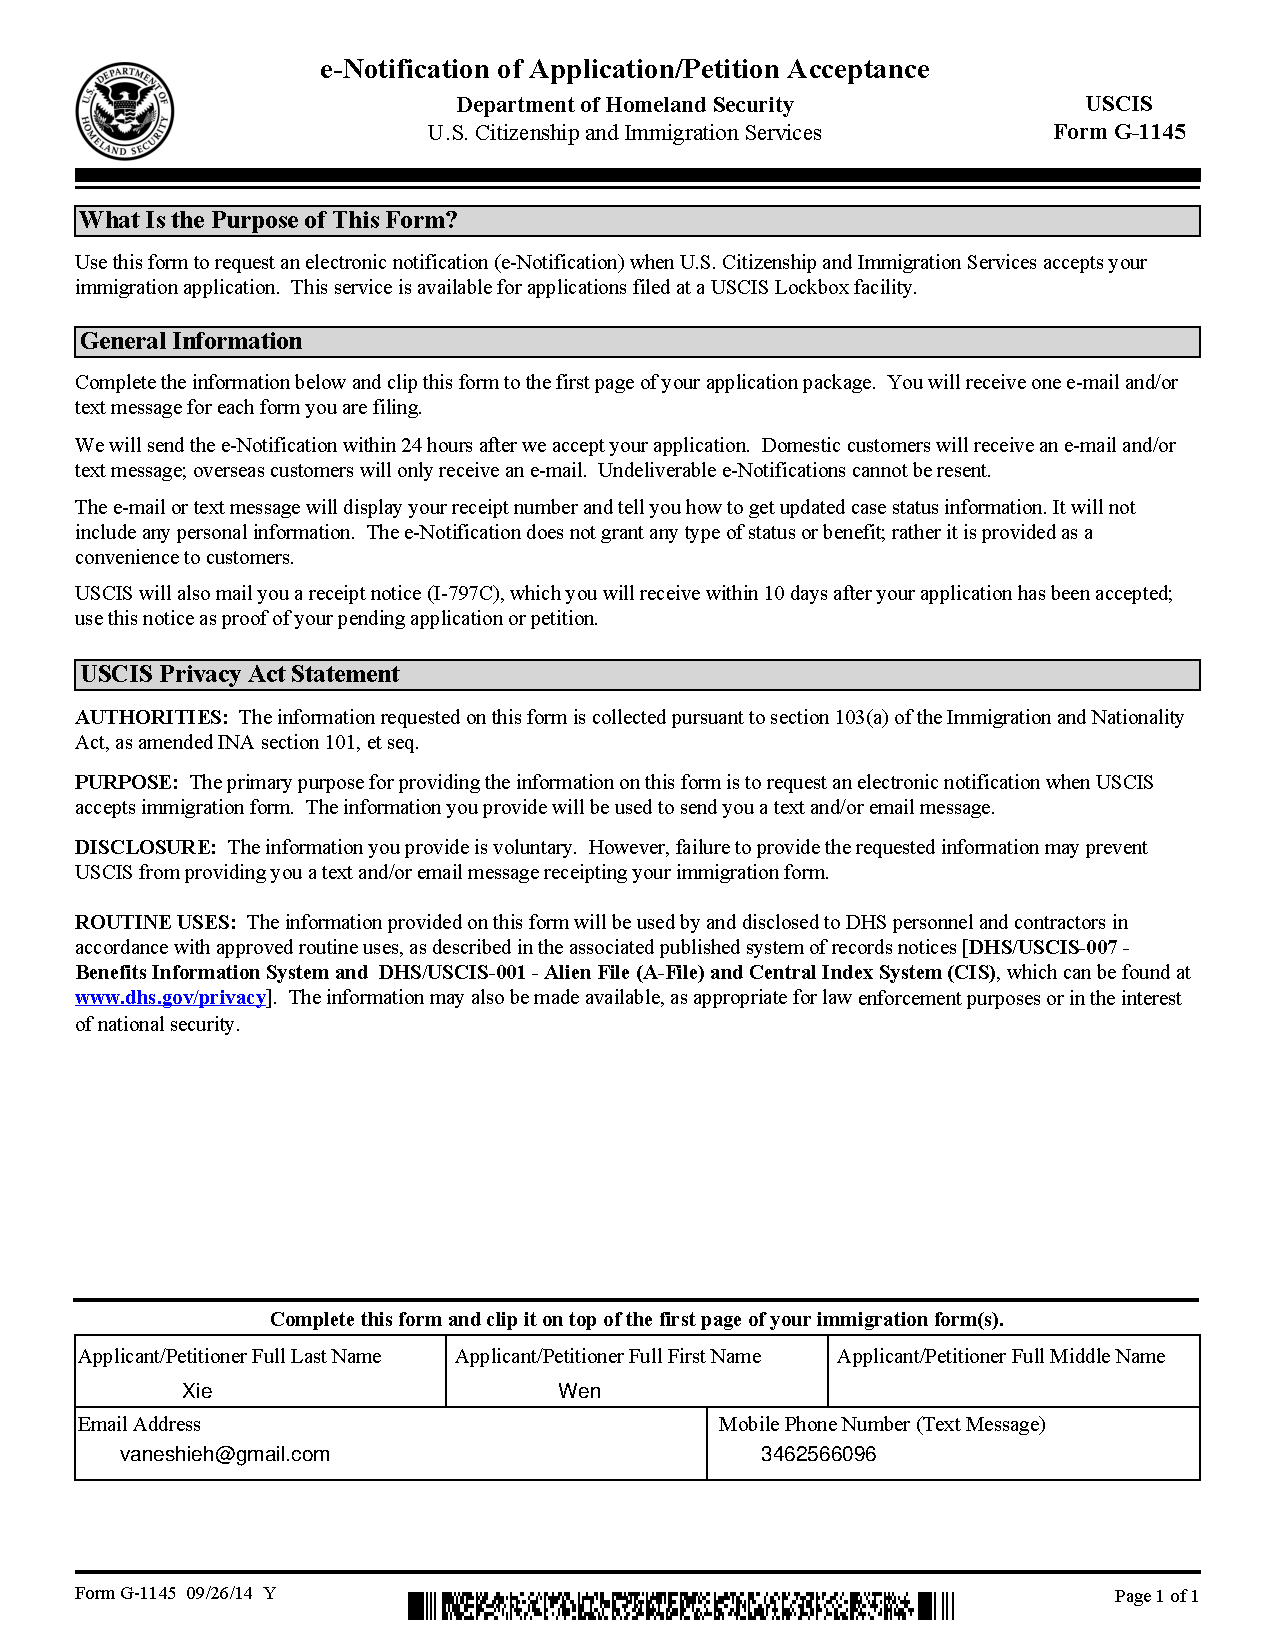
\includepdf[pages=-,pagecommand={},width=1.3\textwidth]{Forms/filled_1145.pdf}

\label{ETA-9089}
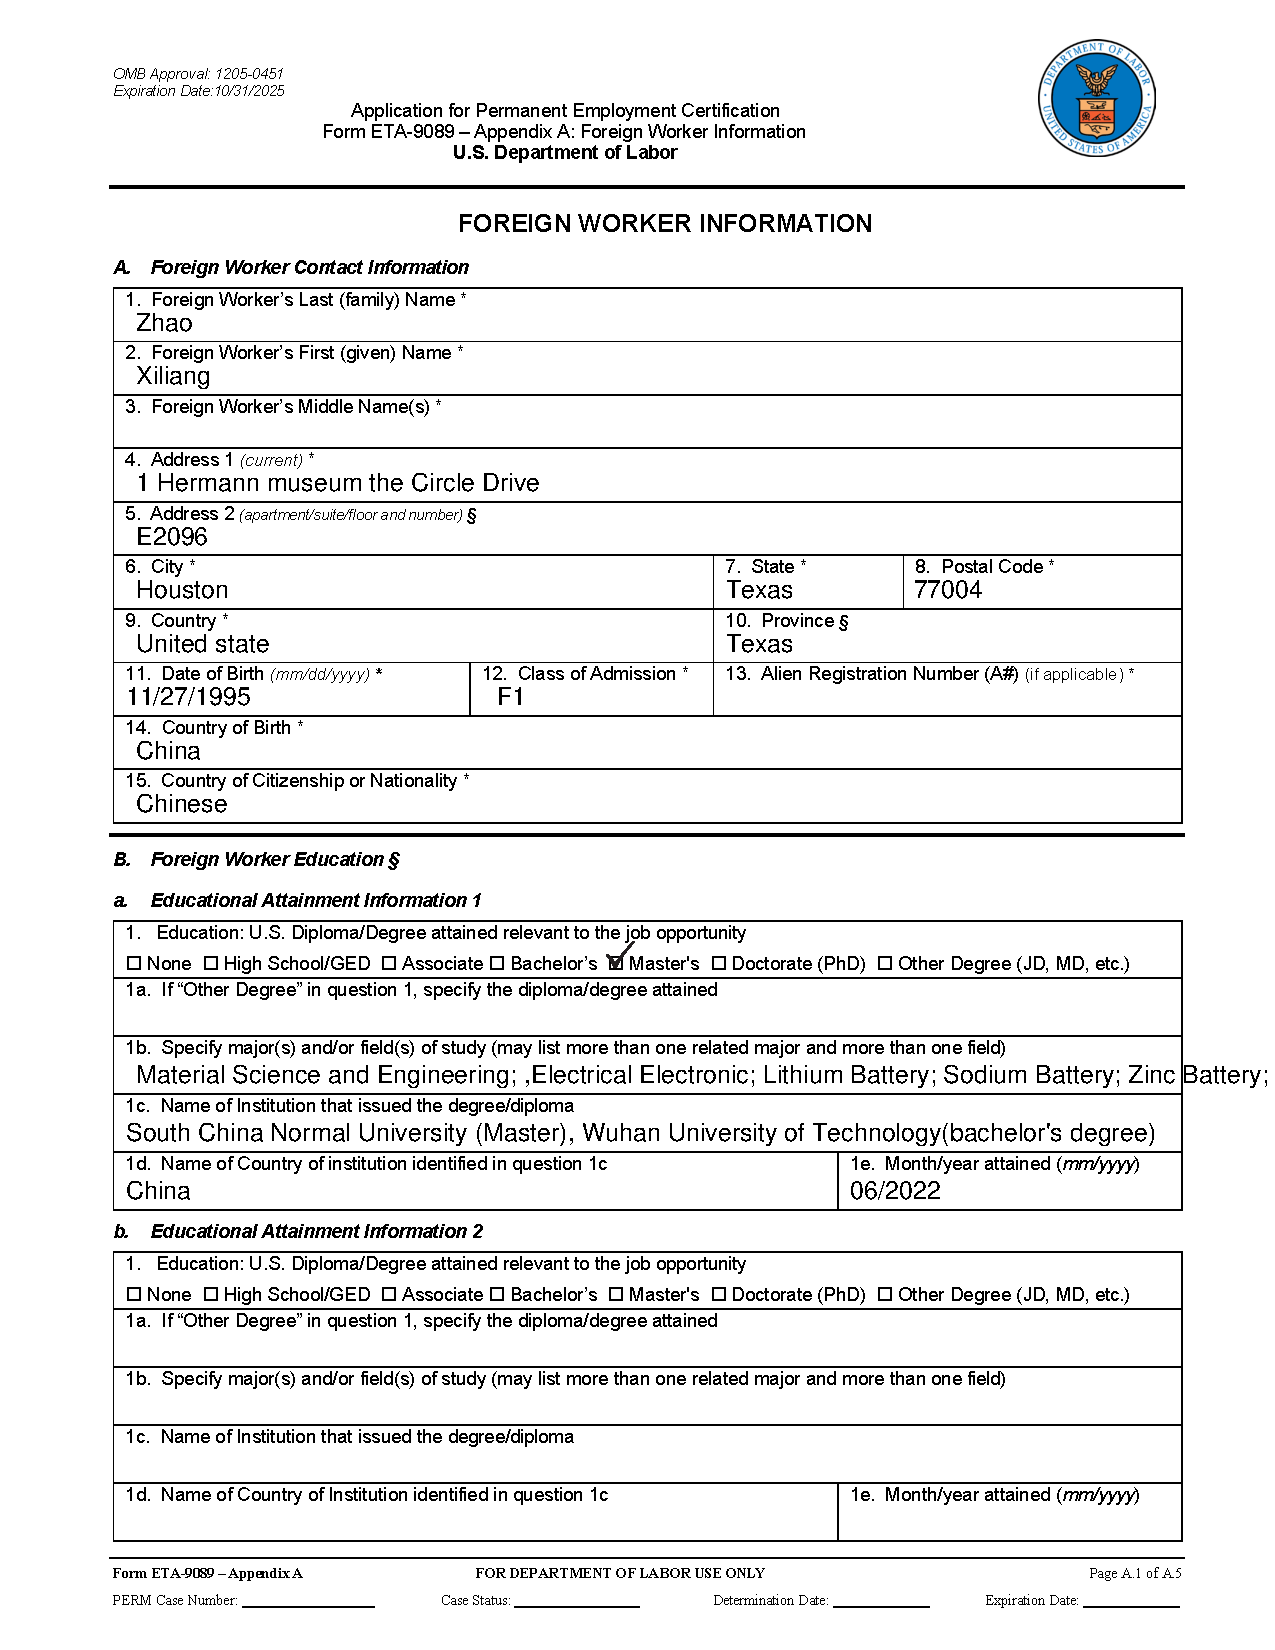
\includepdf[pages=-,pagecommand={},width=1.3\textwidth]{Forms/filled_9089.pdf}


\label{I-140}
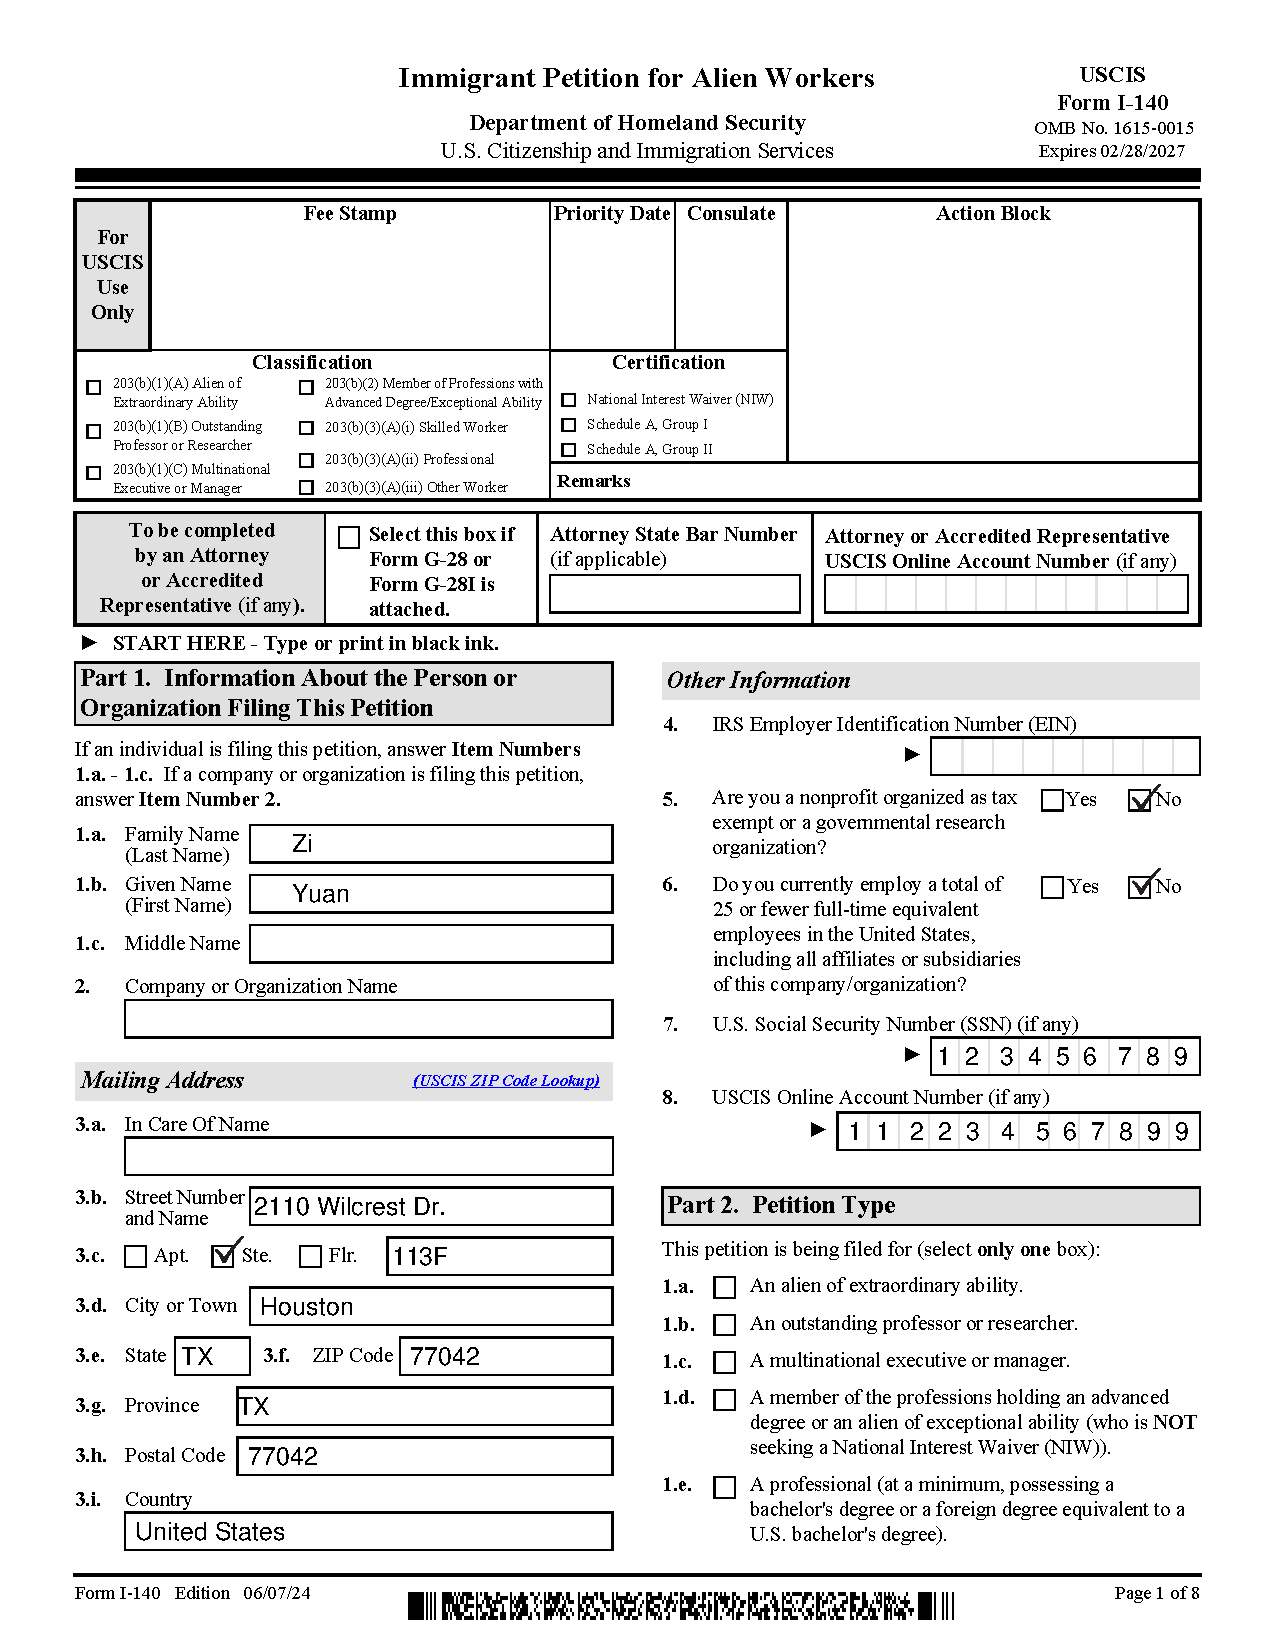
\includepdf[pages=-,pagecommand={},width=1.3\textwidth]{Forms/filled_140.pdf}

\clearpage
July 20, 2025
\label{petition}
\\
2501 S. State Hwy. 121 Business\\
USCIS\\
Lewisville, TX 75067-8003

\underline{\bf EB-2 Petition for Permanent Residency with Request for a National Interest Waiver}

\begin{tabular}{ll}
{\bf Petitioner and Beneficiary:} & Qin Liu \\
{\bf Classification Sought:} & 203(b) (2) NIW\\
{\bf Type of Petition:} & I-140
\end{tabular}
\vspace{2\baselineskip}

Dear Sir/Madam:

This letter is respectfully submitted in support of Dr. Liu's petition for classification as a qualified immigrant worker under the preference of alien of exceptional ability/advanced degree professional. The evidence submitted herein will specifically demonstrate that Dr. Liu qualifies for a National Interest Waiver under the standards set by \textit{Matter of DHANASAR}, 26 I\&N Dec. 884 (AAO 2016).

Specifically, the evidence submitted will prove:
\begin{enumerate}
    \item That Dr. Liu's proposed endeavor has both substantial merit and national importance;
    \item That Dr. Liu is well positioned to advance the proposed endeavor; and
    \item That, on balance, it would be beneficial to the United States to waive the requirement of a job offer and thus of a labor certification.
\end{enumerate}

\clearpage





{\bf \underline{Section 1.} DR. Liu'S BACKGROUND AND ACHIEVEMENTS}

The following is an overview of Dr. Liu's unique and exceptional background and his outstanding contributions to his field. This overview will serve as part of the basis for how Dr. Liu is in a field of substantial intrinsic merit and national importance, and how Dr. Liu is well-positioned to advance his proposed endeavors. It will also serve as part of the basis for why, on balance, it is beneficial to the United States to waive a job offer requirement, and thus a labor certification.

{\bf 1.1 Dr. Liu's Exceptional Educational Background and Work Experience}

Dr. Liu is an outstanding researcher and engineer who has made significant contributions to the fields of None, particularly in machine learning, artificial intelligence, AI Safety \& LLM Reliability, Trustworthy and Ethical AI. As an expert in the field, Dr. Liu's educational background has provided him with the unique ability to contribute significantly to these important research fields.

Originally from China, Dr. Liu obtained a B.A. in Philosophy from Fudan University. Fudan University is a comprehensive and key national university directly under the administration of the the Ministry of Education. It consistently ranks as a leading university in None and is among the top universities in the world in its field. According to the QS World University Rankings (2026), it is placed at 30 worldwide and 3 in China. For philosophy, QS places Fudan University in the 41 range globally. In the field of philosophy, which Dr. Liu studied, Fudan University ranks 5 nationally in China.

After graduating from Fudan University, Dr. Liu enrolled in Fudan University and received his M.S. in Computer Science in 2022. Fudan University is a comprehensive public research university research university and the 4 university in Shanghai, China. QS, in its third-year PhD ranking of National Universities, ranked Fudan University 5 and in its Best Value Schools ranked it N/A.

Currently, Dr. Liu works as a PhD student at University of California, Davis, located in Davis, California. Founded in 1905, University of California, Davis has established itself as a leading provider of education technology, offering services including UC Davis provides nationally important services in health, agriculture, and education, with growing national impact in computer science and artificial intelligence. The university supports cutting-edge research in AI safety, machine learning, natural language processing, and cybersecurity through its Computer Science Department and interdisciplinary institutes. Faculty and PhD students actively contribute to federally funded research on trustworthy AI, human-centered computing, and responsible data science, helping shape national policy and safety standards. UC Davis also plays a key role in training the next generation of computer scientists through NSF-funded programs, AI4ALL outreach, and undergraduate research initiatives that broaden participation in STEM. These efforts complement its nationally recognized work in public health (e.g., the UC Davis Medical Center and MIND Institute), global disease surveillance (One Health Institute), and sustainable agriculture (UC ANR). Together, UC Davis’s contributions in computing and beyond advance critical national priorities in technology, safety, public health, and education.. With its operations spanning UC Davis operates across multiple regions in California, extending its impact far beyond its main campus. The central campus in Davis serves as the academic and research hub, housing core programs in computer science, engineering, and life sciences. In nearby Sacramento, the UC Davis Medical Center provides advanced clinical care and telemedicine services, serving communities across the state. The university also maintains specialized research facilities in diverse ecological regions, including the Tahoe Environmental Research Center in Lake Tahoe and the Bodega Marine Laboratory on the northern California coast. Its School of Veterinary Medicine extends into Southern California, offering clinical services and outreach. Additionally, through the UC Agriculture and Natural Resources (UC ANR) division, UC Davis supports Cooperative Extension offices and agricultural research centers across nearly every California county. These distributed operations allow UC Davis to contribute statewide to public health, sustainable agriculture, environmental science, and advanced computing research., University of California, Davis delivers a broad range of solutions—including UC Davis offers nationally impactful solutions in computer science, particularly in the areas of artificial intelligence, natural language processing, cybersecurity, and responsible computing. Faculty and research labs contribute cutting-edge work on AI safety, large language model (LLM) reliability, and human-centered machine learning—addressing urgent national priorities related to trustworthy and ethical AI deployment. UC Davis researchers also develop tools for robust NLP systems, algorithmic fairness, privacy-preserving computation, and secure software infrastructure, many of which are supported by federal agencies such as the NSF, NIH, and DARPA.  The university plays a leadership role in advancing national research agendas through interdisciplinary centers and collaborations that connect computer science with public health, law, and environmental science. UC Davis also supports workforce development through its graduate and undergraduate CS programs, and broadens national participation in computing through initiatives like AI4ALL and inclusive CS education partnerships. These efforts collectively ensure that UC Davis is not only advancing the frontier of computing research, but also shaping how AI and digital technologies are safely and equitably integrated into society at a national scale.—backed by dedicated technical support and customer service. Employing approximately 24,000 professionals and generating an estimated annual revenue of \$\$7.3 billion, University of California, Davis's global footprint underscores its commitment to delivering advanced and reliable services to the None industry.

The fact that Dr. Liu remains in top-tier universities/companies reflects his outstanding academic and research credentials. The meaning of his work is not limited to the benefits of the people of N/A but to the interests of the American people as a whole. Below is only a sampling of his major contributions to the field.



{\bf 1.2. Dr. Liu's Original Contributions to computer science and artificial intelligence and Its Applications in Information Technology}

The Information Technology depends on computer science and artificial intelligence to The primary purpose of my field—artificial intelligence and trustworthy natural language processing—is to develop safe, reliable, and transparent AI systems that serve the public good and support national priorities. As large language models and AI technologies are increasingly integrated into sectors like healthcare, education, law, defense, and public infrastructure, ensuring their safety, robustness, and alignment with human values is critical. My work focuses on advancing methods to detect and mitigate harmful or unintended AI behaviors, improve model interpretability, and establish standards for responsible deployment. This contributes to national goals by enhancing the security, ethical use, and trustworthiness of AI systems, while supporting innovation and maintaining U.S. leadership in emerging technologies.. Achieving this goal requires None. Traditional methods, however, often struggle with To address the core challenges in trustworthy AI and NLP—particularly those your research tackles—the field must advance in several key directions:  **1. Strengthen Alignment and Robustness Techniques** Large language models often exhibit unsafe or unintended behaviors under adversarial or ambiguous prompts. Addressing this requires scalable alignment strategies such as reward modeling, denoised product-of-experts, and multi-turn red teaming, all of which are central themes in your work.  **2. Enhance Evaluation Beyond Standard Benchmarks** Traditional accuracy metrics fail to capture risks related to misuse, hallucination, or misalignment. The field needs fine-grained, safety-focused evaluation protocols—including behavioral auditing, context-sensitive testing, and attack success rate analysis—which your research actively advances.  **3. Improve Resilience Against Jailbreaks and Unsafe Prompting** LLMs remain vulnerable to prompt-based exploits. Tackling this requires deeper understanding of representation-level vulnerabilities and robust, model-internal safety filters. Your work contributes by diagnosing and mitigating such failures through backdoor defense and probing mechanisms.  **4. Design Scalable Oversight and Monitoring Systems** As models grow in size and capability, continuous post-deployment oversight becomes essential. This includes real-time output monitoring, interpretability tools, and methods for detecting emergent unsafe behaviors—areas where your framework-level contributions are especially relevant.  **5. Build Foundations for Human-AI Trust and Governance** To ensure responsible integration of AI into sensitive domains, the field must integrate human-in-the-loop systems, enforceable alignment guarantees, and policy-aware design principles. Your research helps define how LLMs can be steered and evaluated in complex, real-world settings.  Together, these directions reflect not only the field’s priorities but also the concrete problems my publications seek to address—advancing the reliability, safety, and societal alignment of next-generation language technologies.. These shortcomings can lead to None.

Dr. Liu's research addresses these challenges by merging None with cutting-edge tools in None. her work focuses on enhancing the safety, reliability, transparency, and robustness of large language models and AI systems, ultimately improving how we develop AI responsibly, safeguard against misuse, support high-stakes decision-making, and inform technology policy. In her investigations of  safety alignment and failure modes in large language model systems, she explores how large language models can exhibit unsafe or misaligned behavior under benign or adversarial inputs, especially when researchers must analyze numerous possibilities for emergent unsafe behaviors that are difficult to predict, reproduce, or formally verify. Accurate AI systems' safeness and robustness against adversarial user inputs is critical for the safe and reliable deployment of AI systems in high-stakes national domains such as healthcare, education, public policy, and security.

To better understand and analyze the behavior and reliability of large language models, researchers collect data such as model outputs, internal representations, failure cases, and adversarial user inputs.. training-time defenses, inference-time interventions, and representation-level manipulations stands out as a powerful method for diagnosing, mitigating, and preventing unsafe or misaligned behaviors in large language models and AI systems, generating detailed alignment risk profiles, adversarial vulnerabilities, and behavioral failure patterns. Traditional training-time defenses, inference-time interventions, and representation-level manipulations, however, faces limitations when the lack of reliable methods to anticipate and generalize model behavior across diverse real-world contexts, potentially causing undetected safety failures, poor robustness under distribution shifts, and vulnerability to adversarial or manipulative inputs in high-stakes deployments. Dr. Liu addressed these issues by developing LLM knowledge access control framework named SudoLM, which regulates internal knowledge activation in large language models to preserve safety alignment and prevent unauthorized behavior.. she also created a denoised product-of-experts (PoE) defense framework based on ensembled training to mitigate backdoor attacks in large language models by suppressing malicious triggers while preserving benign task performance., maintaining critical robust filtering of adversarial or misaligned data signals during training and evaluation and improving model alignment, safety consistency, and resistance to backdoor or prompt-based attacks..

Further advancing her research, Dr. Liu developed ensembles-based training optimization framework to enhance improving the robustness and safety alignment of large language models. Given the importance of  deploying AI systems in nationally sensitive domains such as healthcare, law, and defense where reliability and trust are paramount, she designed authorization-aligned model knowledge access control strategy that addresses unauthorized knowledge activation and misaligned behavior in large language models, thereby ensuring safer, more controllable AI systems suitable for deployment in critical national domains such as healthcare, law, and public infrastructure.. To improve LLM knowledge access control, she combined authorization-aligned policy learning with key-based routing and inference-time supervision to ensure controlled and modular knowledge activation in large language models. for Direct Preference Optimization (DPO), utilizing synthetic and real-world datasets to minimize misalignment errors and unauthorized knowledge activation across large language model instruction following and access control..

In the field of AI policy and governance, Dr. Liu implemented authorization-based Direct Preference Optimization to effectively ensuring that language models respond in ways aligned with authorized user intent, thereby supporting safe and responsible AI deployment in nationally critical sectors, achieving improved alignment consistency, reduced unauthorized behavior, and enhanced control over language model responses. This enhancement of safer AI deployment, increased trustworthiness in high-stakes applications, and stronger safeguards against misuse strengthens the effectiveness of the safe, controllable, and responsible deployment of large language models in service of national interests across healthcare, education, public policy, and security..

Additionally, her research extends to Vision–Language Model safety, where the challenge of safety degradation caused by modality shifts and cross-modal interactions that can trigger unsafe or misaligned responses in multi-modal AI systems. must be addressed efficiently and accurately. To solve this challenge, she developed inference-time representation manipulation system (CMRM) that automates restoring safety alignment in vision–language models without requiring additional training, significantly improving workflow efficiency while enhancing accuracy in ensuring the safety and alignment of large language and vision–language models.

All of Dr. Liu's methodologies have been extensively validated using both cross-modal adversarial image–text pairs and vision–language safety benchmarks, consistently demonstrating superior performance compared to conventional approaches in terms of unsafe response rate reduction, alignment preservation under modality shifts, and robustness against adversarial image–text inputs. her work has gained significant recognition and has been published in leading journals, including 1. Secrets of rlhf in large language models part i: Ppo; 2. Textflint: Unified multilingual robustness evaluation toolkit for natural language processing; 3. Muirbench: A comprehensive benchmark for robust multi-image understanding; 4. Flooding-X: Improving BERT’s resistance to adversarial attacks via loss-restricted fine-tuning; 5. From shortcuts to triggers: Backdoor defense with denoised poe; 6. Test-time backdoor mitigation for black-box large language models with defensive demonstrations; 7. Securing multi-turn conversational language models from distributed backdoor attacks; 8. Unraveling and mitigating safety alignment degradation of vision-language models; 9. Monotonic paraphrasing improves generalization of language model prompting; 10. Metascale: Test-time scaling with evolving meta-thoughts; 11. Sudolm: Learning access control of parametric knowledge with authorization alignment. By advancing the frontiers of computer science and artificial intelligence through alignment-aware large language models and vision–language intervention techniques, Dr. Liu's contributions enable more safer, more reliable, and resilient to misuse in high-stakes national applications practices in Information Technology.









{\bf 1.3 Dr. Liu's Unique Expertise and International Reputation in the Field }

During the course of her excellent research experience, Dr. Liu has developed an exceptional repertoire of knowledge and skills. In addition to her strong basic science background that spans artificial intelligence, natural language processing, machine learning security, and vision–language modeling, she has mastered many cutting-edge techniques. These techniques include but are not limited to preference optimization, adversarial evaluation, backdoor defense, prompt-based alignment, model knowledge access control, and zero-shot generalization. All this expertise paved the way for Dr. Liu to make contributions to her dedicated fields of Artificial Intelligence, Natural Language Processing, Machine Learning Security, and Trustworthy Computing. Moreover, Dr. Liu has the scientific acumen to develop new techniques and models by employing her interdisciplinary training, knowledge, and skills to address practical problems.

Furthermore, Dr. Liu's past excellent experience has perfectly prepared her for her current challenging and interdisciplinary research. In summary, Dr. Liu's strong background and unique skills will enable her to make greater progress in her current work than few others are capable of (\textbf{Exhibits 0-5}). Below is a summary of Dr. Liu's exceptional achievements.

{\bf 1.3.1 Dr. Liu's Outstanding Publication and Citation Record}

Dr. Liu's exceptional research results have been published in \textbf{26 papers} in top-notch journals and conferences (\textbf{Exhibits 1-5}). These journals and conferences are at the top of the field and only those original and significant discoveries can be published.

\textbf{MUIRBENCH: A COMPREHENSIVE BENCHMARK FOR ROBUST MULTI-IMAGE UNDERSTANDING} aims to bridge the gap between technology, methodologies, and scientific understanding in Computer Vision and Multimodal Machine Learning, by publishing explicitly written articles intelligible to researchers and engineers working in any field of Developing systematic evaluation frameworks for assessing the robustness, generalization, and reasoning capabilities of AI models in multi-image understanding tasks.. It has a 2025 impact factor of \textbf{304}.

\textbf{TextFlint: Unified Multilingual Robustness Evaluation Toolkit for Natural Language Processing} focuses on natural language processing with emphasis on Natural Language Processing robustness evaluation and toolkit development.. According to the Journal Citation Reports, the journal had a 2025 impact factor of \textbf{215}.

\textbf{Flooding-X: Improving BERT’s Resistance to Adversarial Attacks via Loss-Restricted Fine-Tuning} publishes research in Natural Language Processing (NLP) robustness with applications in Enhancing the adversarial robustness of BERT by introducing a training-time regularization method (Flooding-X) that improves resistance to textual adversarial attacks without added computational cost.. The journal's 2015 impact factor is \textbf{215}.

\textbf{From Shortcuts to Triggers: Backdoor Defense with Denoised PoE} covers advances in  NLP model robustness with focus on defending against adversarial backdoor attacks using a novel denoised product-of-experts approach. The journal emphasizes Mitigating backdoor vulnerabilities in NLP models by separating malicious trigger learning from clean task learning through a denoised product-of-experts framework..

\textbf{Monotonic Paraphrasing Improves Generalization of Language Model Prompting} promotes research in Natural Language Processing robustness and prompt engineering aimed at Developing and evaluating an end-to-end decoding strategy that systematically rewrites prompts into lower-perplexity paraphrases—without additional training—to enhance zero-shot generalization on unseen tasks and instructions..

Additionally, according to Google Scholar, Dr. Liu's work has been cited 634 times by her peers (\textbf{Exhibit 6}). her research has been referenced in review and research papers that prioritize citing the most recent advances. These citations come from scientists in a wide range of countries and territories, highlighting the global impact and relevance of her work.

Notable citing regions include \textbf{United States}, \textbf{China}, \textbf{United Kingdom}, \textbf{Singapore}, and \textbf{Australia}. The citations originate from researchers affiliated with world-renowned institutions such as \textbf{University of Waterloo, Tsinghua University, Sea AI Lab}, \textbf{Zhejiang University, Nanyang Technological University, Shanghai Jiao Tong University, National University of Singapore}, \textbf{Facebook AI, Stanford University}, \textbf{Sun Yat-sen University, Guangxi University, Guangdong Key Laboratory of Big Data Analysis and Processing, Key Laboratory of Machine Intelligence and Advanced Computing}, and \textbf{University of Virginia, Virginia Tech, University of Maryland, College Park, Merck \& Co., Inc., University of Georgia}.

In addition to academic institutions, industry leaders such as \textbf{Google}, \textbf{Microsoft}, \textbf{Meta}, \textbf{Apple}, and \textbf{NVIDIA} have acknowledged Dr. Liu's contributions. This widespread recognition underscores the international influence and application of Dr. Liu's research, which continues to drive advancements across various sectors and regions.








{\bf 1.3.2 Dr. Liu's Research Achievements Have Been Widely Cited and Emphasized by Prestigious Reviews and Original Research Articles}

Normally, only the most important advances in the field are cited and emphasized in review or original research articles. Dr. Liu's studies have been cited by many review and research articles. For example:
\begin{enumerate}[label=• ]
    \item In a research paper titled "\textit{Mantis: Interleaved Multi-Image Instruction Tuning}" published in \textit{Transactions on Machine Learning Research} by researchers from University of Waterloo, Tsinghua University, Sea AI Lab, Dr. Liu's work was cited: "\textit{MuirBench (Wang et al., 2024a) is a comprehensive benchmark consisting of 12 diverse multi-image tasks, such as scene understanding, ordering, etc. It contains 2,600 multiple-choice questions with 11,264 images involved in total. We report the overall average performance across the 12 tasks.}" (\textbf{Exhibit 7}).

    \item In a paper titled "\textit{Defending LVLMs Against Vision Attacks Through Partial-Perception Supervision}" published in \textit{International Conference on Machine Learning} by authors from Zhejiang University, Nanyang Technological University, Shanghai Jiao Tong University, National University of Singapore, Dr. Liu's research was referenced: "\textit{However, research indicates that LVLMs demonstrate weaker defense performance compared to LLMs (Liu et al., 2024c). }" (\textbf{Exhibit 8}).

    \item In a study titled "\textit{Dynaboard: An Evaluation-As-A-Service Platform for Holistic Next-Generation Benchmarking}" published in \textit{Conference on Neural Information Processing Systems} by scientists at Facebook AI, Stanford University, they highlighted Dr. Liu's contributions: "\textit{That is, following past work on NLP robustness [30, 31], we perturb examples and measure whether a model’s prediction changes. Specifically, we use the recently released TextFlint5 evaluation toolkit [24] to do so (details are provided in Appendix B). ; We thank the TextFlint team for their help on the toolkit. }" (\textbf{Exhibit 9}).

    \item In research published as "\textit{RMLM: A Flexible Defense Framework for Proactively Mitigating Word-level Adversarial Attacks}" in \textit{Annual Meeting of the Association for Computational Linguistics} by researchers from Sun Yat-sen University, Guangxi University, Guangdong Key Laboratory of Big Data Analysis and Processing, Key Laboratory of Machine Intelligence and Advanced Computing, they cited Dr. Liu's findings: "\textit{Flooding-X (Liu et al., 2022) improves Flooding (Ishida et al., 2020) to boost model generalization by preventing further reduction of the training loss.; Compared to the state-of-the-art method Flooding-X across all vic- tim models and datasets ; Further, it can achieve performance on par with Flooding-X when enabling the transformation, while only incurring a slight increase in computational overhead.; Flooding-X. We use the original hyperparam- eters setting in their paper (Liu et al., 2022) of BERT model.}" (\textbf{Exhibit 10}).

    \item In a paper titled "\textit{MIND CONTROL THROUGH CAUSAL INFERENCE: PRE- DICTING CLEAN IMAGES FROM POISONED DATA}" published in \textit{International Conference on Learning Representations} by authors from University of Virginia, Virginia Tech, University of Maryland, College Park, Merck \& Co., Inc., University of Georgia, they referenced Dr. Liu's work: "\textit{(1) The structure is much smaller than SFRN, as backdoor patterns are simpler to learn than normal patterns, as evidenced by (Liu et al., 2023b; Zhang et al., 2023); Firstly, the AIN is intentionally designed to have a much smaller structure than the SFRN, as backdoor patterns are simpler and quicker to learn than normal patterns, as evidenced by prior work (Liu et al., 2023b; Zhang et al., 2023; Yu et al., 2022; Sandoval-Segura et al., 2022).}" (\textbf{Exhibit 11}).
\end{enumerate}




In summary, the fact that many reviews and original research papers cited Dr. Liu's studies to explain their theories or results proves that Dr. Liu's works have significantly influenced her dedicated fields and inspired many new research directions for her peers.







{\bf \underline{Section 2.} DR. Liu QUALIFIES FOR A NATIONAL INTEREST WAIVER}

{\bf 2.1 Dr. Liu's Proposed Endeavor Has Both Substantial Merit and National Importance}

Dr. Liu's proposed endeavor to advance research in artificial intelligence, natural language processing, machine learning security, and vision–language modeling and artificial intelligence and national security industries. demonstrates both substantial merit and national importance through concrete evidence of impact and recognition. With over 0, still in PhD program years of dedicated research experience, Dr. Liu has established herself as a leading expert in preference optimization, adversarial robustness, backdoor defense, prompt-based alignment, access control in language models, zero-shot generalization, and vision–language model safety., as demonstrated by her extensive publication record and citation impact.

The substantial merit of Dr. Liu's work is evidenced by publications in prestigious journals including MUIRBENCH: A COMPREHENSIVE BENCHMARK FOR ROBUST MULTI-IMAGE UNDERSTANDING, TextFlint: Unified Multilingual Robustness Evaluation Toolkit for Natural Language Processing, and Flooding-X: Improving BERT’s Resistance to Adversarial Attacks via Loss-Restricted Fine-Tuning, which are leading venues in their respective fields with impact factors of 304, 215, and 215. The national importance of this research is further validated by 634 citations from renowned institutions including University of Waterloo, Tsinghua University, Sea AI Lab, Zhejiang University, Nanyang Technological University, Shanghai Jiao Tong University, National University of Singapore, and Facebook AI, Stanford University, as well as industry leaders like Google and Microsoft. This widespread adoption across both academic and commercial sectors demonstrates the practical value and broad applicability of Dr. Liu's innovations.

The national importance of Dr. Liu's work is particularly evident in its direct alignment with critical U.S. priorities in secure AI deployment, innovation leadership, and the safe integration of advanced technologies into essential public services.. her research bridges theoretical innovation with practical applications, providing scalable solutions for artificial intelligence and national security industries. that enhance U.S. technological leadership and economic competitiveness. The geographic diversity of citations from United States, China, and United Kingdom further demonstrates the global impact and significance of this work.

Dr. Liu's unique ability to integrate machine learning, natural language processing, adversarial robustness, and AI policy and governance. has produced transformative contributions that address pressing challenges in AI misuse and disinformation, technological safety and alignment, digital trust and security, and the governance of advanced AI systems.. her innovative approaches to ensuring the safety, realibility, and robustness of large language and vision–language models in real-world, high-stakes deployments. have established new methodologies that advance both scientific understanding and practical implementation. This work directly contributes to maintaining U.S. leadership in artificial intelligence, natural language processing, machine learning, vision–language modeling, and trustworthy computing while addressing critical national priorities in energy efficiency, environmental protection, and sustainable development.

The substantial merit and national importance of Dr. Liu's endeavors are evident through her significant research contributions and their direct alignment with key U.S. priorities. Through continued advancement of her research program, Dr. Liu is positioned to generate lasting benefits that align with and advance vital U.S. interests in artificial intelligence, natural language processing, machine learning, vision–language modeling, and trustworthy computing and artificial intelligence and national security industries..



{\bf 2.2 Dr. Liu is Well Positioned to Advance her Research}

As discussed in Section 1, Dr. Liu holds a M.S. in Computer Science from Fudan University, and has extensive research experience in artificial intelligence, natural language processing, machine learning, vision–language modeling, and trustworthy computing. Dr. Liu has published 26 influential articles in the fields of her endeavors, and her papers have been cited 634 times and implemented by scientists from around the world (\textbf{Exhibits 1-5}). Dr. Liu has frequently been invited as a peer reviewer for many scientific journals (\textbf{Exhibit 12}). her education, experience, and expertise in her field, the significance of her role in research projects position her well to advance her proposed endeavor in artificial intelligence, natural language processing, machine learning, vision–language modeling, and trustworthy computing.

Dr. Liu's unique combination of technical expertise, innovative thinking, and real-world application makes her exceptionally well-positioned to continue advancing her field. This is evidenced by the extensive citations of her work in leading journals (\textbf{Exhibits 6-7}). her innovative research, exceptional achievements, and commitment to addressing critical global challenges have resulted in groundbreaking advancements in artificial intelligence, natural language processing, machine learning, vision–language modeling, and trustworthy computing, with lasting benefits for the nation and beyond, as demonstrated by the widespread adoption of her methodologies (\textbf{Exhibits 8-11}).

What sets Dr. Liu apart is her interdisciplinary approach, combining machine learning, natural language processing, adversarial robustness, and AI policy and governance. to deliver practical and scalable solutions. her efforts have tangible implications for AI safety and security, public policy support, healthcare decision-making, education technology, and national defense systems.—fields critical to U.S. interests, as evidenced by citations in major research papers (\textbf{Exhibits 9-11}). Dr. Qin Liu's expertise and innovative research continue to benefit the United States, with her work directly addressing national priorities in secure AI deployment, innovation leadership, and the safe integration of advanced technologies into essential public services., making her an invaluable asset to the scientific and technological landscape.

Thus, as is detailed above (Section 1) and demonstrated through extensive citations and research impact (\textbf{Exhibits 6-11}), Dr. Liu has the proven abilities and past accomplishments to suggest that she is well positioned to advance research in artificial intelligence, natural language processing, machine learning, vision–language modeling, and trustworthy computing and the artificial intelligence and national security industries. in the United States.



{\bf 2.3 On Balance, It Is Beneficial to the United States to Waive the Requirements of a Job Offer and Thus of a Labor Certification}

Dr. Liu's record of successful work in artificial intelligence, natural language processing, machine learning, vision–language modeling, and trustworthy computing, and her contributions to the artificial intelligence and national security industries. are of such value that, on balance, would benefit the United States even assuming that other qualified U.S. workers are available. Dr. Liu possesses unique and innovative skills, knowledge, and background that serve the national interest well. she is one of the very rare-to-find scientists, engineers, and business leaders with extensive experience in artificial intelligence, AI safety. she holds a M.S. in Computer Science and has over 0, still in PhD program years of experience in preference optimization, adversarial robustness, backdoor defense, prompt optimization, alignment tuning, access control in language models, red teaming, and vision–language model optimization. Dr. Liu has a broad and unique set of skills, knowledge, and background for her current and future work in the field of artificial intelligence, natural language processing, machine learning, vision–language modeling, and trustworthy computing (see Section 1 above).

On the basic science aspect, Dr. Liu has a strong foundation in fundamental theory and experimental work. she is an expert in the cutting-edge techniques for preference optimization, adversarial evaluation, backdoor defense, prompt optimization, safety alignment, model knowledge access control, and multi-modal model auditing., and is also skilled in the application of machine learning, deep learning, preference optimization to ensuring the safety, realibility, and robustness of large language and vision–language models in real-world, high-stakes deployments.. To find someone so adept at all of the critical skills that Dr. Liu possesses is very difficult. Dr. Liu's unique skills are not only a key factor to her past success, but will enable her to make further contributions in the United States.

Dr. Liu's work directly addresses some of the most pressing challenges in secure AI deployment, innovation leadership, and the safe integration of advanced technologies into essential public services., making her an invaluable asset to both academia and industry. her innovative research integrates cutting-edge methodologies in artificial intelligence, natural language processing, machine learning, vision–language modeling, and trustworthy computing, deep learning, and alignment-aware optimization, which is vital for addressing global challenges such as AI misuse and disinformation, technological safety and alignment, digital trust and security, and the governance of advanced AI systems..

Dr. Liu's consistent discoveries and breakthroughs of high degree and productivity suggest that she is destined to continue making substantial contributions in the field of artificial intelligence, natural language processing, machine learning, vision–language modeling, and trustworthy computing at a degree higher than her peers. Dr. Liu's innovative and novel contributions prove her ability to make unprecedented, unparalleled, and vital contributions to the national interest. she has a truly impressive record of success in machine learning, natural language processing, AI safety,  trustworthy AI systems and has made breakthroughs that are already reaping significant benefits. In addition, she has solved critical problems that have hindered scientists and engineers for years, and her specific contributions to the research are above what can be expected from others with similar education and experience.

As a recent M.S. graduate, she has already achieved a level of expertise and impact that is rare for someone at her career stage. her dedication to advancing scientific knowledge and solving practical problems has earned her recognition from peers and collaborators alike. All of these special qualities, skills, abilities, and knowledge, combined with her extensive background in artificial intelligence, natural language processing, machine learning, vision–language modeling, and trustworthy computing, make Dr. Liu ideally suited to her future research projects in the United States. All of these factors are highly beneficial overall and distinguish Dr. Liu from her peers. Moreover, these unique traits cannot be effectively articulated on a labor certification (\textbf{Exhibits 15-19}).

Furthermore, as discussed above, Dr. Liu's work is important to the economic growth and artificial intelligence and national security industries. of the United States as her research leads to better artificial intelligence, natural language processing, machine learning, vision–language modeling, and trustworthy computing and improved production strategies in artificial intelligence and national security industries.. New advances by Dr. Liu in this area will result in substantial benefits for a wealthier and safer America. The extensive recognition of her work by experts in this field demonstrates that her continuous participation is critical to artificial intelligence, natural language processing, machine learning, vision–language modeling, and trustworthy computing and artificial intelligence and national security industries. (\textbf{Exhibits 13-14}).




\vspace{2\baselineskip}

Qin Liu\\
1710 R ST,\\
Sacramento, CA, 95811\\
Tel. 2137058435
\clearpage

{\bf List of Exhibits}
\label{exhib}

\begin{enumerate}[label={Exhibit \arabic*:}]
    \item Journal or international conference paper co-authored by Dr. Liu 
    \item Journal or international conference paper co-authored by Dr. Liu 
    \item Journal or international conference paper co-authored by Dr. Liu 
    \item Journal or international conference paper co-authored by Dr. Liu 
    \item Journal or international conference paper co-authored by Dr. Liu 
    \item The citation record of Dr. Liu’s papers according to Google Scholar 
    \item Information of the journals where Dr. Liu has published papers 
    \item Original research paper which utilized Dr. Liu’s works 
    \item Original research paper which utilized Dr. Liu’s works 
    \item Original research paper which utilized Dr. Liu’s works  
    \item Original research paper which utilized Dr. Liu’s works 
    \item Original research paper which utilized Dr. Liu’s works 
    \item Evidence that Dr. Liu has served as a peer-reviewer for manuscripts submitted to academic journals
    \item Copy of Dr. Liu’s CV
    \item Copy of Dr. Liu’s Ph.D. diploma
    \item Copy of Dr. Liu’s passport, visa and I-94
    \item Copy of Dr. Liu’s I-20 forms and Employment Authorization Document (EAD) 
    \item Copy of Dr. Liu’s employment verification letter
\end{enumerate}

\clearpage

\vspace*{\fill}

\begin{center}

{\LARGE \bf
Exhibit 1 
}

\vspace{10\baselineskip}

{\large Journal or international conference paper co-authored by Dr. Liu}

\end{center}
\vspace*{\fill}

\includepdf[pages=-,pagecommand={},width=1.3\textwidth]{Exhibits/Exhibit1.pdf}

\vspace*{\fill}

\begin{center}

{\LARGE \bf
Exhibit 2
}

\vspace{10\baselineskip}

{\large Journal or international conference paper co-authored by Dr. Liu}

\end{center}
\vspace*{\fill}

\includepdf[pages=-,pagecommand={},width=1.3\textwidth]{Exhibits/Exhibit2.pdf}

\vspace*{\fill}

\begin{center}

{\LARGE \bf
Exhibit 3
}

\vspace{10\baselineskip}

{\large Journal or international conference paper co-authored by Dr. Liu}

\end{center}
\vspace*{\fill}

\includepdf[pages=-,pagecommand={},width=1.3\textwidth]{Exhibits/Exhibit3.pdf}

\vspace*{\fill}

\begin{center}

{\LARGE \bf
Exhibit 4
}

\vspace{10\baselineskip}

{\large Journal or international conference paper co-authored by Dr. Liu}

\end{center}
\vspace*{\fill}

\includepdf[pages=-,pagecommand={},width=1.3\textwidth]{Exhibits/Exhibit4.pdf}

\vspace*{\fill}

\begin{center}

{\LARGE \bf
Exhibit 5
}

\vspace{10\baselineskip}

{\large Journal or international conference paper co-authored by Dr. Liu}

\end{center}
\vspace*{\fill}

\includepdf[pages=-,pagecommand={},width=1.3\textwidth]{Exhibits/Exhibit5.pdf}


\vspace*{\fill}

\begin{center}

{\LARGE \bf
Exhibit 6
}

\vspace{10\baselineskip}

{\large The citation record of Dr. Liu’s papers according to Google Scholar}

\end{center}
\vspace*{\fill}

\includepdf[pages=-,pagecommand={},width=1.3\textwidth]{Exhibits/Exhibit6.pdf}

\vspace*{\fill}

\begin{center}

{\LARGE \bf
Exhibit 7
}

\vspace{10\baselineskip}

{\large Information of the journals where Dr. Liu has published papers }

\end{center}
\vspace*{\fill}

\includepdf[pages=-,pagecommand={},width=1.3\textwidth]{Exhibits/Exhibit7.pdf}

\vspace*{\fill}

\begin{center}

{\LARGE \bf
Exhibit 8
}

\vspace{10\baselineskip}

{\large Original research paper which utilized Dr. Liu’s works}

\end{center}
\vspace*{\fill}

\includepdf[pages=-,pagecommand={},width=1.3\textwidth]{Exhibits/Exhibit8.pdf}

\vspace*{\fill}

\begin{center}

{\LARGE \bf
Exhibit 9
}

\vspace{10\baselineskip}

{\large Original research paper which utilized Dr. Liu’s works}

\end{center}
\vspace*{\fill}

\includepdf[pages=-,pagecommand={},width=1.3\textwidth]{Exhibits/Exhibit9.pdf}

\vspace*{\fill}

\begin{center}

{\LARGE \bf
Exhibit 10
}

\vspace{10\baselineskip}

{\large Original research paper which utilized Dr. Liu’s works}

\end{center}
\vspace*{\fill}

\includepdf[pages=-,pagecommand={},width=1.3\textwidth]{Exhibits/Exhibit10.pdf}

\vspace*{\fill}

\begin{center}

{\LARGE \bf
Exhibit 11
}

\vspace{10\baselineskip}

{\large Original research paper which utilized Dr. Liu’s works}

\end{center}
\vspace*{\fill}

\includepdf[pages=-,pagecommand={},width=1.3\textwidth]{Exhibits/Exhibit11.pdf}

\vspace*{\fill}

\begin{center}

{\LARGE \bf
Exhibit 12
}

\vspace{10\baselineskip}

{\large Original research paper which utilized Dr. Liu’s works}

\end{center}
\vspace*{\fill}

\includepdf[pages=-,pagecommand={},width=1.3\textwidth]{Exhibits/Exhibit12.pdf}



\vspace*{\fill}

\begin{center}

{\LARGE \bf
Exhibit 13
}

\vspace{10\baselineskip}

{\large Evidence that Dr. Liu has served as a peer-reviewer for manuscripts submitted to academic journals}

\end{center}
\vspace*{\fill}

\includepdf[pages=-,pagecommand={},width=1.3\textwidth]{Exhibits/Exhibit13.pdf}



\vspace*{\fill}

\begin{center}

{\LARGE \bf
Exhibit 14
}

\vspace{10\baselineskip}

{\large Copy of Dr. Liu’s CV}

\end{center}
\vspace*{\fill}

\includepdf[pages=-,pagecommand={},width=1.3\textwidth]{Exhibits/Exhibit14.pdf}

\vspace*{\fill}

\begin{center}

{\LARGE \bf
Exhibit 15
}

\vspace{10\baselineskip}

{\large Copy of Dr. Liu’s Ph.D. diploma}

\end{center}
\vspace*{\fill}

\includepdf[pages=-,pagecommand={},width=1.3\textwidth]{Exhibits/Exhibit15.pdf}

\vspace*{\fill}

\begin{center}

{\LARGE \bf
Exhibit 16
}

\vspace{10\baselineskip}

{\large Copy of Dr. Liu’s passport, visa and I-94}

\end{center}
\vspace*{\fill}

\includepdf[pages=-,pagecommand={},width=1.3\textwidth]{Exhibits/Exhibit16.pdf}

\vspace*{\fill}

\begin{center}

{\LARGE \bf
Exhibit 17
}

\vspace{10\baselineskip}

{\large Copy of Dr. Liu’s I-20 forms and Employment Authorization Document (EAD)}

\end{center}
\vspace*{\fill}

\includepdf[pages=-,pagecommand={},width=1.3\textwidth]{Exhibits/Exhibit17.pdf}

\vspace*{\fill}

\begin{center}

{\LARGE \bf
Exhibit 18
}

\vspace{10\baselineskip}

{\large Copy of Dr. Liu’s employment verification letter}

\end{center}
\vspace*{\fill}

\includepdf[pages=-,pagecommand={},width=1.3\textwidth]{Exhibits/Exhibit18.pdf}

\vspace*{\fill}



\end{document}